\documentclass[12pt,a4paper]{article}

\setlength{\topmargin}{0.0in}
\setlength{\oddsidemargin}{0.33in}
\setlength{\textheight}{9.0in}
\setlength{\textwidth}{6.0in}
\renewcommand{\baselinestretch}{1.25}

\usepackage[backend=bibtex,style=numeric,sorting=none]{biblatex}
\usepackage{amsmath}
\usepackage{amsfonts}
\usepackage{graphicx}
\usepackage{float}
\usepackage{subcaption}

\addbibresource{ref.bib}

\title{Title of Special Topic}
\author{Lecture Course}
\date{Candidate Number: xxxxxx}

\begin{document}

\maketitle

\thispagestyle{empty}

\newpage
\setcounter{page}{1}



\begin{abstract}
  Insert some waffle here if you want. Abstracts are optional for
  special topics but are part of page count.
\end{abstract}

\section{Introduction}
In this paper, we aim to find robust methods to solve highly anisotropic diffusion problems. Thus we want to solve

\begin{equation}
\begin{cases}
-\nabla \cdot (\mathbb{A}\nabla u) = f, & \text{ in }\Omega,\\
\mathbf{n}\cdot \mathbb{A}\nabla u = 0, & \text{ on }\Gamma_N, \\
u = g, & \text{  on }\Gamma_D,
\end{cases}
\end{equation}
where
\begin{equation}
\mathbb{A} = \epsilon^{-1} A_{||}\mathbf{b}\otimes \mathbf{b}
+(I - \mathbf{b}\otimes \mathbf{b})\mathbb{A}_{\perp}
(I - \mathbf{b}\otimes \mathbf{b}).
\end{equation}
    Here $\epsilon \ll 1$ is the anisotropic coefficient. And $|\mathbf{b}|=1$ with $\mathbf{b}$ representing the magnetic field.
State restriction on the b

From multiple papers the best notation for this problem is stated in \cite{} \cite{}. Thus we will use a similar notation. 

Talk about problem (problem from not being well posed.)

Say $\Lambda_{in}$ can be any part of stream line


For a scaler feild $u\in\mathbb{R}$ and vector field $v \in \mathbb{R}^d$, we use the notation
\begin{align}
v_{||} &=(\mathbf{b} \otimes \mathbf{b})v = (v \cdot \mathbf{b})\mathbf{b}
, & v_{\perp} &= (\mathbb{I}-\mathbf{b} \otimes \mathbf{b})v,\\
\nabla_{||}u &= (\mathbf{b} \otimes \mathbf{b}) \nabla u = (\nabla u \cdot \mathbf{b})\mathbf{b},
& \nabla_{\perp} u &= (\mathbb{I}-\mathbf{b} \otimes \mathbf{b}) \nabla u,\\
\nabla_{||} \cdot u &= \nabla \cdot u_{||},
& \nabla_{\perp} \cdot u &= \nabla \cdot u_{\perp}.
\end{align}
Now we define 
\begin{align}
\Delta_{||}u &= \nabla_{||}\cdot(A_{||}\nabla_{||}u)  =
\nabla \cdot(A_{||} (\mathbf{b} \otimes \mathbf{b}) \nabla u)\\
\Delta_{\perp}u  &= \nabla_{\perp}\cdot(\mathbb{A}_{\perp}\nabla_{\perp}u)  = 
\nabla \cdot((\mathbb{I}-\mathbf{b} \otimes \mathbf{b})\mathbb{A}_{\perp}(\mathbb{I}-\mathbf{b} \otimes \mathbf{b})\nabla u)
\end{align}

Thus from \ref{} and \ref{} it is clear to see \ref{} can be written as
\begin{align}
\mathbb{A} \nabla u = 
\varepsilon^{-1}(A_{||}\nabla_{||} u)_{||} + 
(\mathbb{A}_{\perp}\nabla_{\perp}u)_{\perp} \\
 \\
\end{align}
Thus putting \ref{} into the PDE \ref{} we get
\begin{equation}
\begin{cases}
-\varepsilon^{-1} \Delta_{||}u - \Delta_{\perp}u = f, & \text{ in }\Omega,\\
\mathbf{n}\cdot \mathbb{A}\nabla u = 0, & \text{ on }\Gamma_N, \\
u = g, & \text{  on }\Gamma_D,
\end{cases}
\end{equation}

With the equation (\ref{}) being equal because
\begin{equation}
\nabla_{||}\cdot(A_{||}\nabla_{||}u) = 
\nabla \cdot (A_{||})_{||} 
\end{equation}
can be done as $A_{||}$ is scalar
and (\ref{}) being equal because 

We can now write the PDE \ref{} in weak form

\begin{align}
a_{||}(\alpha, \beta) &= \int_{\Omega} A_{||} \nabla_{||}\alpha \cdot \nabla_{||}\beta d\mathbf{x} \\
a_{\perp}(\alpha, \beta) &= \int_{\Omega}(\mathbb{A}_{\perp} \nabla_{\perp}\alpha )\cdot \nabla_{\perp} \beta d\mathbf{x}
\end{align}
This can be easily calculated in firedrake using
CODESNIP

By splitting up the PDE \ref{} into parts parrelle and perpendicular to the vector feild we get the PDE 

b repressents column vector 
Now we will define all the spaces we will be using

Need to explain why this is a problem

Now we assume $b$ is perp to lam_N and $b$ parralle to lam_D

It should be noted that that ___ are a lot easier to discretise. ()

\section{Overview Of Current Methods}
For these methods and for the numerical simulations in section \ref{} we will take the boundary conditions
\begin{equation}
\begin{cases}
\mathbf{n}\cdot \mathbb{A}\nabla u = 0, & \text{ on }\Gamma_N, \\
u = g, & \text{  on }\Gamma_D.
\end{cases}
\end{equation}

\subsection{Singular Pertubation Method} \label{SP}
The single pertubation method involves solving the weak form of equation \ref{}. Therefore we have a trial function $u \in $ and a test function $\psi \in$. Thus we solve the weak form (\ref{}) for $(u) \in $.
\begin{equation}
(SP)
\begin{cases}
\varepsilon^{-1}a_{||}(u, \psi) + a_{\perp}(u, \psi) = \int_{\Omega} f \psi d\mathbf{x}
\end{cases}
\end{equation}
This method excells for when $\varepsilon$ is normal size

\subsection{Limit Method} \label{LM}
We now introduce a limit method discussed in paper \cite{}. The limit method involves solving the the equation \ref{} when $\varepsilon \rightarrow 0$. This leads to solving the weak form \ref{} for the trial functions $(u, q) \in $ 
\begin{equation}
(LM)
\begin{cases}
a_{\perp}(u, \hat{u}) + a_{||}(q, \hat{u}) = \int_{\Omega} f \hat{u} d\mathbf{x}, 
&\forall \hat{u} \in \\
a_{||}(u, \hat{q}) = 0, & \forall \hat{q} \in 
\end{cases}
\end{equation}

where $(\hat{u}, \hat{q}) \in $ are test functions.

\subsection{MMAP Method} \label{MMAP}
We now introduce a Micro-Macro Asymptotic-Preserving method discussed in paper \cite{}. This method is similar to the $(LM)$ method from section \ref{LM} but from the additional $\varepsilon$ term it is able to deal with $\varepsilon \approx 1$. This leads to solving the weak form \ref{} for the trial functions $(u, q) \in $ 
\begin{equation}
(MMAP)
\begin{cases}
a_{\perp}(u, \hat{u}) + a_{||}(q, \hat{u}) = \int_{\Omega} f \hat{u} d\mathbf{x}, 
&\forall \hat{u} \in \\
a_{||}(u, \hat{q}) - \varepsilon a_{||}(q, \hat{q}) = 0, & \forall \hat{q} \in 
\end{cases}
\end{equation}

where $(\hat{u}, \hat{q}) \in $ are test functions.

\subsection{AP Method} \label{AP}
We now discuss an Asymptotic-Preserving method stated in paper \cite{}. This method involves solving the weak form (\ref{}) for trial functions $(p, \lambda, q, \ell, \mu) \in $

\begin{equation}
(AP)
\begin{cases}
a_{\perp}(p, \eta)+a_{\perp}(q, \eta) + a_{||}(\eta, \lambda) &= \int_{\Omega}f \eta d\mathbf{x},
\\
 a_{||}(p, \kappa) &= 0, 
 \\
 a_{||}(q, \xi) + \varepsilon a_{\perp}(p+q, \xi) &= 
 \int_{\Omega} (\varepsilon f -\ell)\xi d\mathbf{x},
 \\
 a_{||}(\chi, \mu) + \int_{\Omega}q \chi d\mathbf{x} &= 0,
 \\
 a_{||}(\ell, \tau) &= 0,
 \\
\end{cases}
\end{equation}
where $(\eta, \kappa, \xi, \chi, \tau)\in$ are test functions.


\subsection{Limit Stabilisation Method} \label{LM_STAB}
The $(LM)$ method stated in section \ref{LM} struggles when there is a magnetic field $\mathbf{b}$ with closed lines. Thus we introduce a stabilisation method which is discussed in \cite{}. We implement this modification to get the weak form
\begin{equation}
(LM\_STAB)
\begin{cases}
a_{\perp}(u, \hat{u}) + a_{||}(q, \hat{u}) = \int_{\Omega} f \hat{u} d\mathbf{x}, 
&\forall \hat{u} \in \\
a_{||}(u, \hat{q}) = \sigma \int_{\Omega} q \hat{q} d\mathbf{x}, & \forall \hat{q} \in 
\end{cases}
\end{equation}
We solve for trial functions $(u, q) \in $ with test functions $(\hat{u}, \hat{q}) \in $. Say what sigma is proportional too

\subsection{MMAP Stabilisation Method} \label{MMAP_STAB}
\begin{equation}
(MMAP\_STAB)
\begin{cases}
a_{\perp}(u, \hat{u}) + a_{||}(q, \hat{u}) = \int_{\Omega} f \hat{u} d\mathbf{x}, 
&\forall \hat{u} \in \\
a_{||}(u, \hat{q}) - \varepsilon a_{||}(q, \hat{q}) = \sigma \int_{\Omega} q \hat{q} d\mathbf{x}, & \forall \hat{q}\in 
\end{cases}
\end{equation}

\subsection{Deluzet-Narski Method} \label{DN}
This method turns the strongly anisotropic equation into two mildly anisotropic equations to be solved by iteration. This method is stated in \cite{}. This introduces $\varepsilon_0 \gg \varepsilon$ and gives the weak form \ref{} which solves for the sequence of trial functions $(u^{(n)}, q^{(n)}) \in $ .
 \begin{equation}
 (DN)
   \begin{cases}
  a_{||}(u, \hat{u}) + \varepsilon_0 a_{\perp}(u, \hat{u}) = 
  \varepsilon_0 \int_{\Omega} f \hat{u} d\mathbf{x}
  +(\varepsilon-\varepsilon_0)a_{||}(q, \hat{u}),
  & \forall \hat{u} \in \\
  a_{||}(q, \hat{q}) + \varepsilon_0 a_{\perp}(q, \hat{q}) = 
  \int_{\Omega} f \hat{q} d\mathbf{x}
  -a_{\perp}(u - \varepsilon_0 q, \hat{q}),
  & \forall \hat{q} \in 
  \end{cases}
  \end{equation}
With test functions $(\hat{u}, \hat{q}) \in \mathcal{V} \times \mathcal{V}$.

\section{New Method}
We introduce a new method based on unpublished notes from Patrick Farrell \cite{}. 
By doing the substitution $q=\varepsilon^{-1} \mathbf{b} \cdot \nabla u$ into (\ref{}) we get the weak form
\begin{equation}
(PF)
\begin{cases}
\int_{\Omega}A_{||}q\mathbf{b} \cdot \nabla \hat{u}  d\mathbf{x} + a_{\perp}(u, \hat{u}) 
= \int{\Omega} f \hat{u} d\mathbf{x},
\\
\int_{\Omega}\mathbf{b} \cdot \nabla \hat{u}\hat{q} d\mathbf{x} 
= \varepsilon \int_{\Omega}q\hat{q} d \mathbf{x}, 
\end{cases}
\end{equation}
We solve for trial function with test functions . Also, after some algebraic manipulation 
\begin{align}
q &= \varepsilon^{-1} \mathbf{b}\cdot \nabla u\\
q &= \varepsilon^{-1} \mathbf{b} \cdot \nabla_{||} u \\
\mathbf{b}q &= \varepsilon^{-1} \nabla_{||} u 
\end{align}
Additionally, we can use the stabilisation technique stated in \cite{} to get the weak form
\begin{equation}
(PF\_STAB)
\begin{cases}
\int_{\Omega}A_{||}q\mathbf{b} \cdot \nabla \hat{u}  d\mathbf{x} + a_{\perp}(u, \hat{u}) 
= \int{\Omega} f \hat{u} d\mathbf{x},
\\
\int_{\Omega}\mathbf{b} \cdot \nabla \hat{u}\hat{q} d\mathbf{x} 
= (\varepsilon + \sigma)\int_{\Omega}q\hat{q} d \mathbf{x}, 
\end{cases}
\end{equation}

\section{Derivation Of Current Methods}
It is important to understand the derivation of the current methods because the techniques used ...



\section{Numerical Demonstrations}
In these examples we calculate $f$ from passing $u$ through the PDE.
\subsection{Example 1}
We will solve the PDE (\ref{}) with $\Omega = [0,1]^2, \Gamma_D = \{y=0 \text{ or } y=1\}$ and $\Gamma_N = \{x=0 \text{ or } x=1\}$. We chose a magnetic field such
\begin{equation} \label{E1_b}
\mathbf{b} = \frac{\mathbf{B}}{|\mathbf{B}|}, 
\mathbf{B} = \left[ \begin{matrix}
\alpha(2y-1)cos(m\pi x) + \pi\\
\pi \alpha m (y^2-y)sin(m \pi x)
\end{matrix} \right]
\end{equation}
Thus we have $\Gamma_{in} := \{x=0\}$ and exact solution
\begin{equation}
u = \sin(\pi y + \alpha (y^2-y) \cos(m\pi x)) + \varepsilon \cos(2 \pi x) \sin(\pi y)
\end{equation}
We will cover three sub-examples with $(\alpha=0),(\alpha=2,m=1)$ and $(\alpha = 2, m=10)$. Thus we get electromagnetic fields  shown in Figure \ref{E1_VFs}. The field for $\alpha = 0$ is not shown as it is a simple vector field with $\mathbf{b}= [1, 0]$.
\begin{figure}[H]
 \begin{subfigure}{0.5\textwidth}
     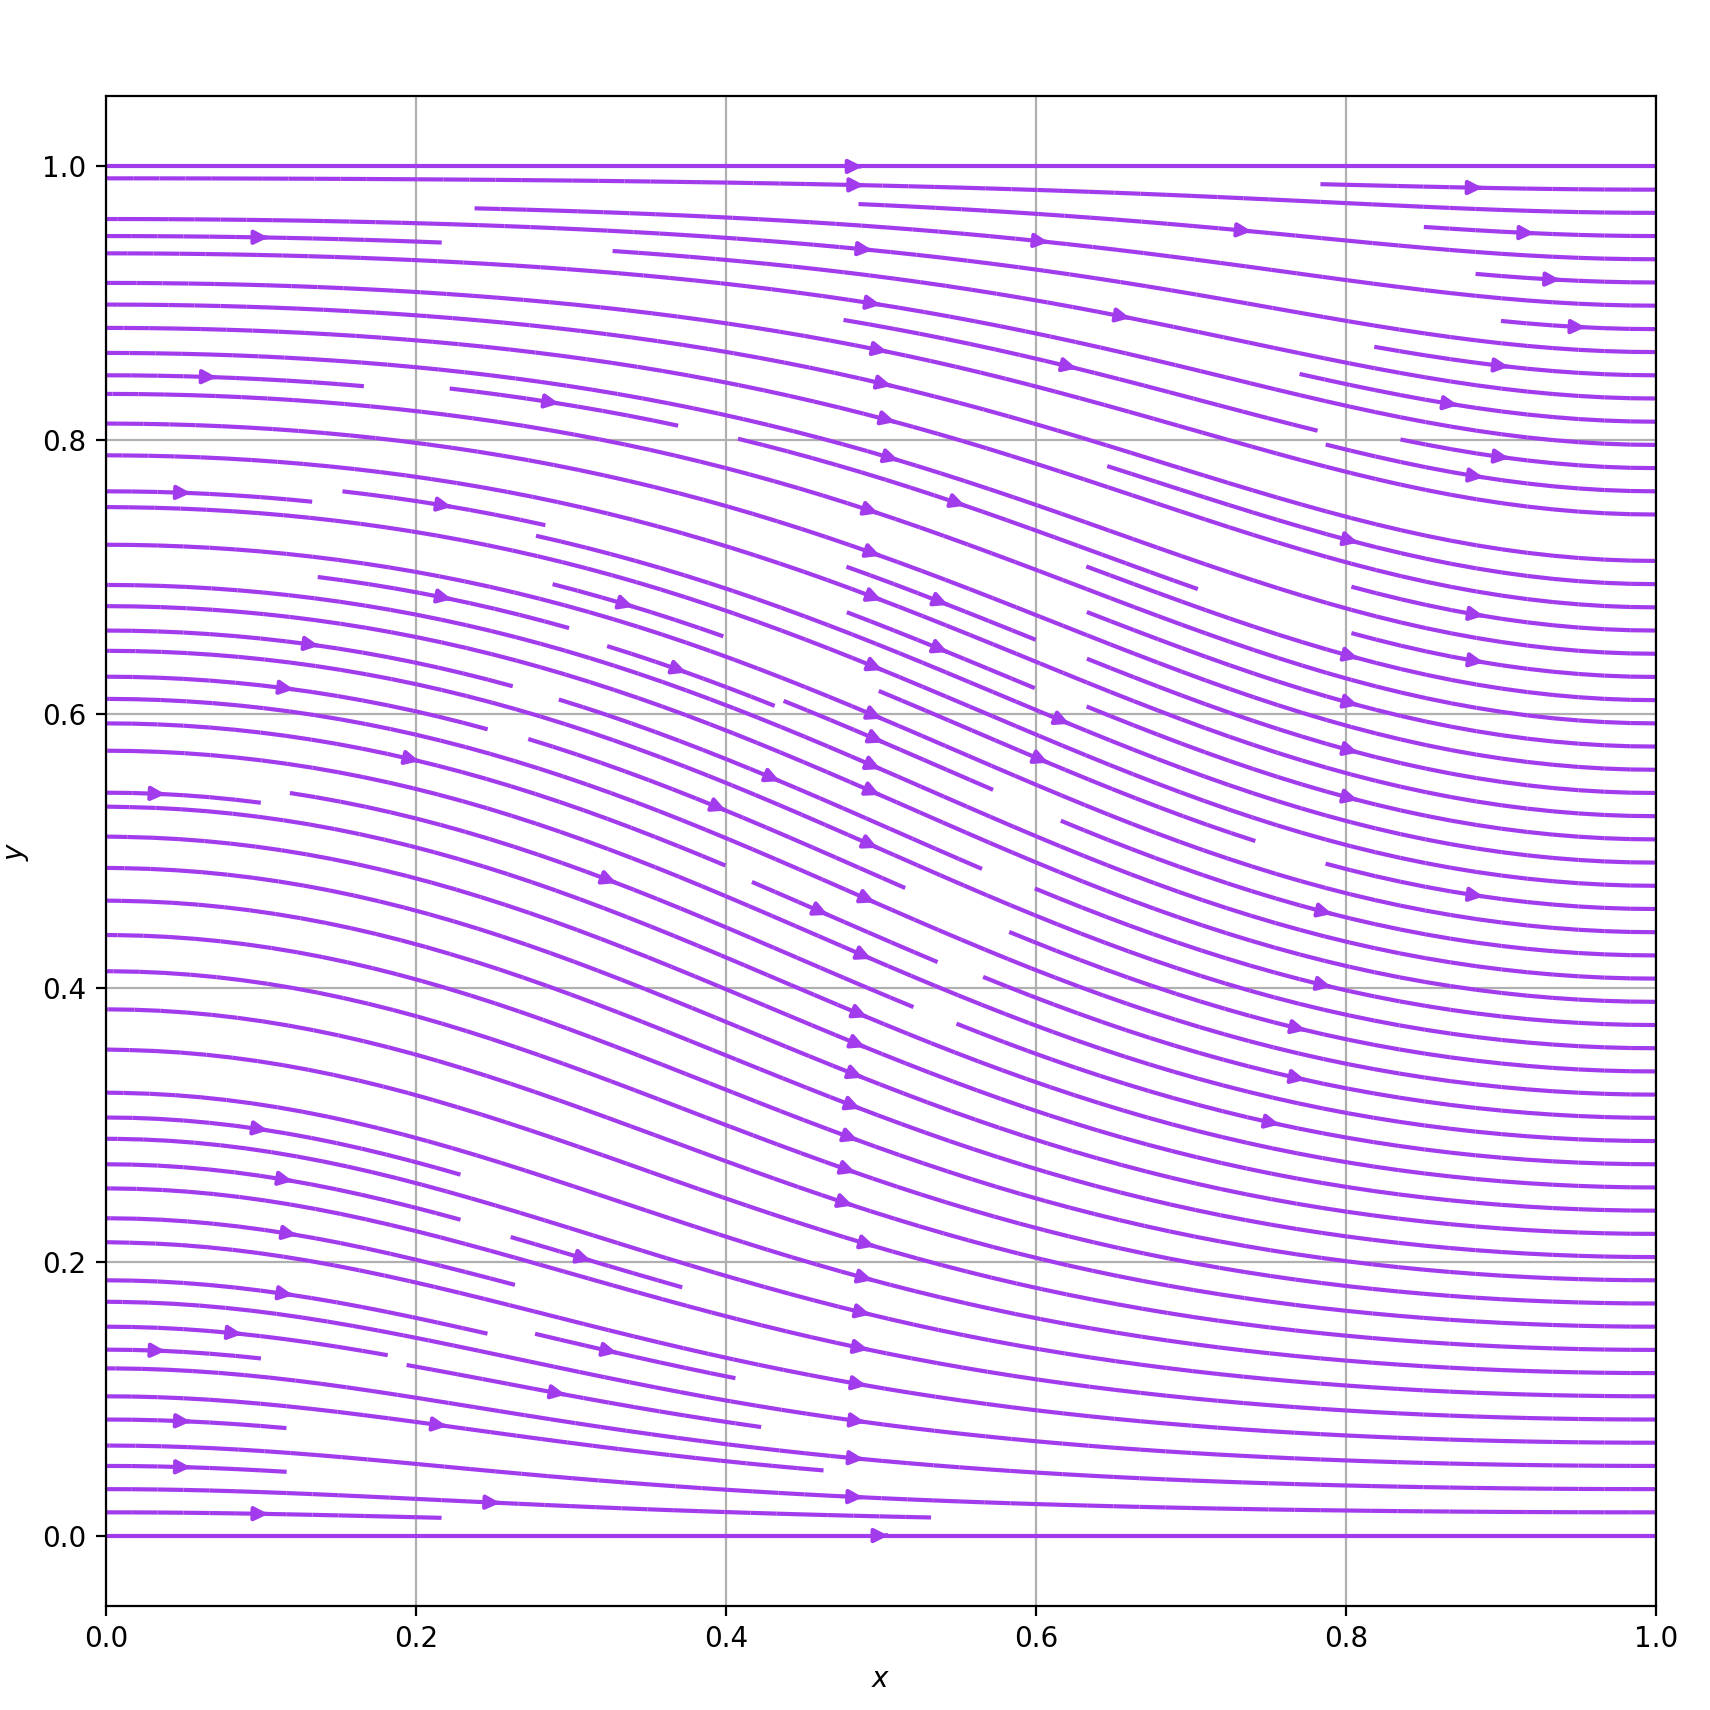
\includegraphics[width=\textwidth]{Pics/VectorField/E1b_a2_m1.png}
     \caption{$\alpha=2, m=1$}
 \end{subfigure}
   \begin{subfigure}{0.5\textwidth}
     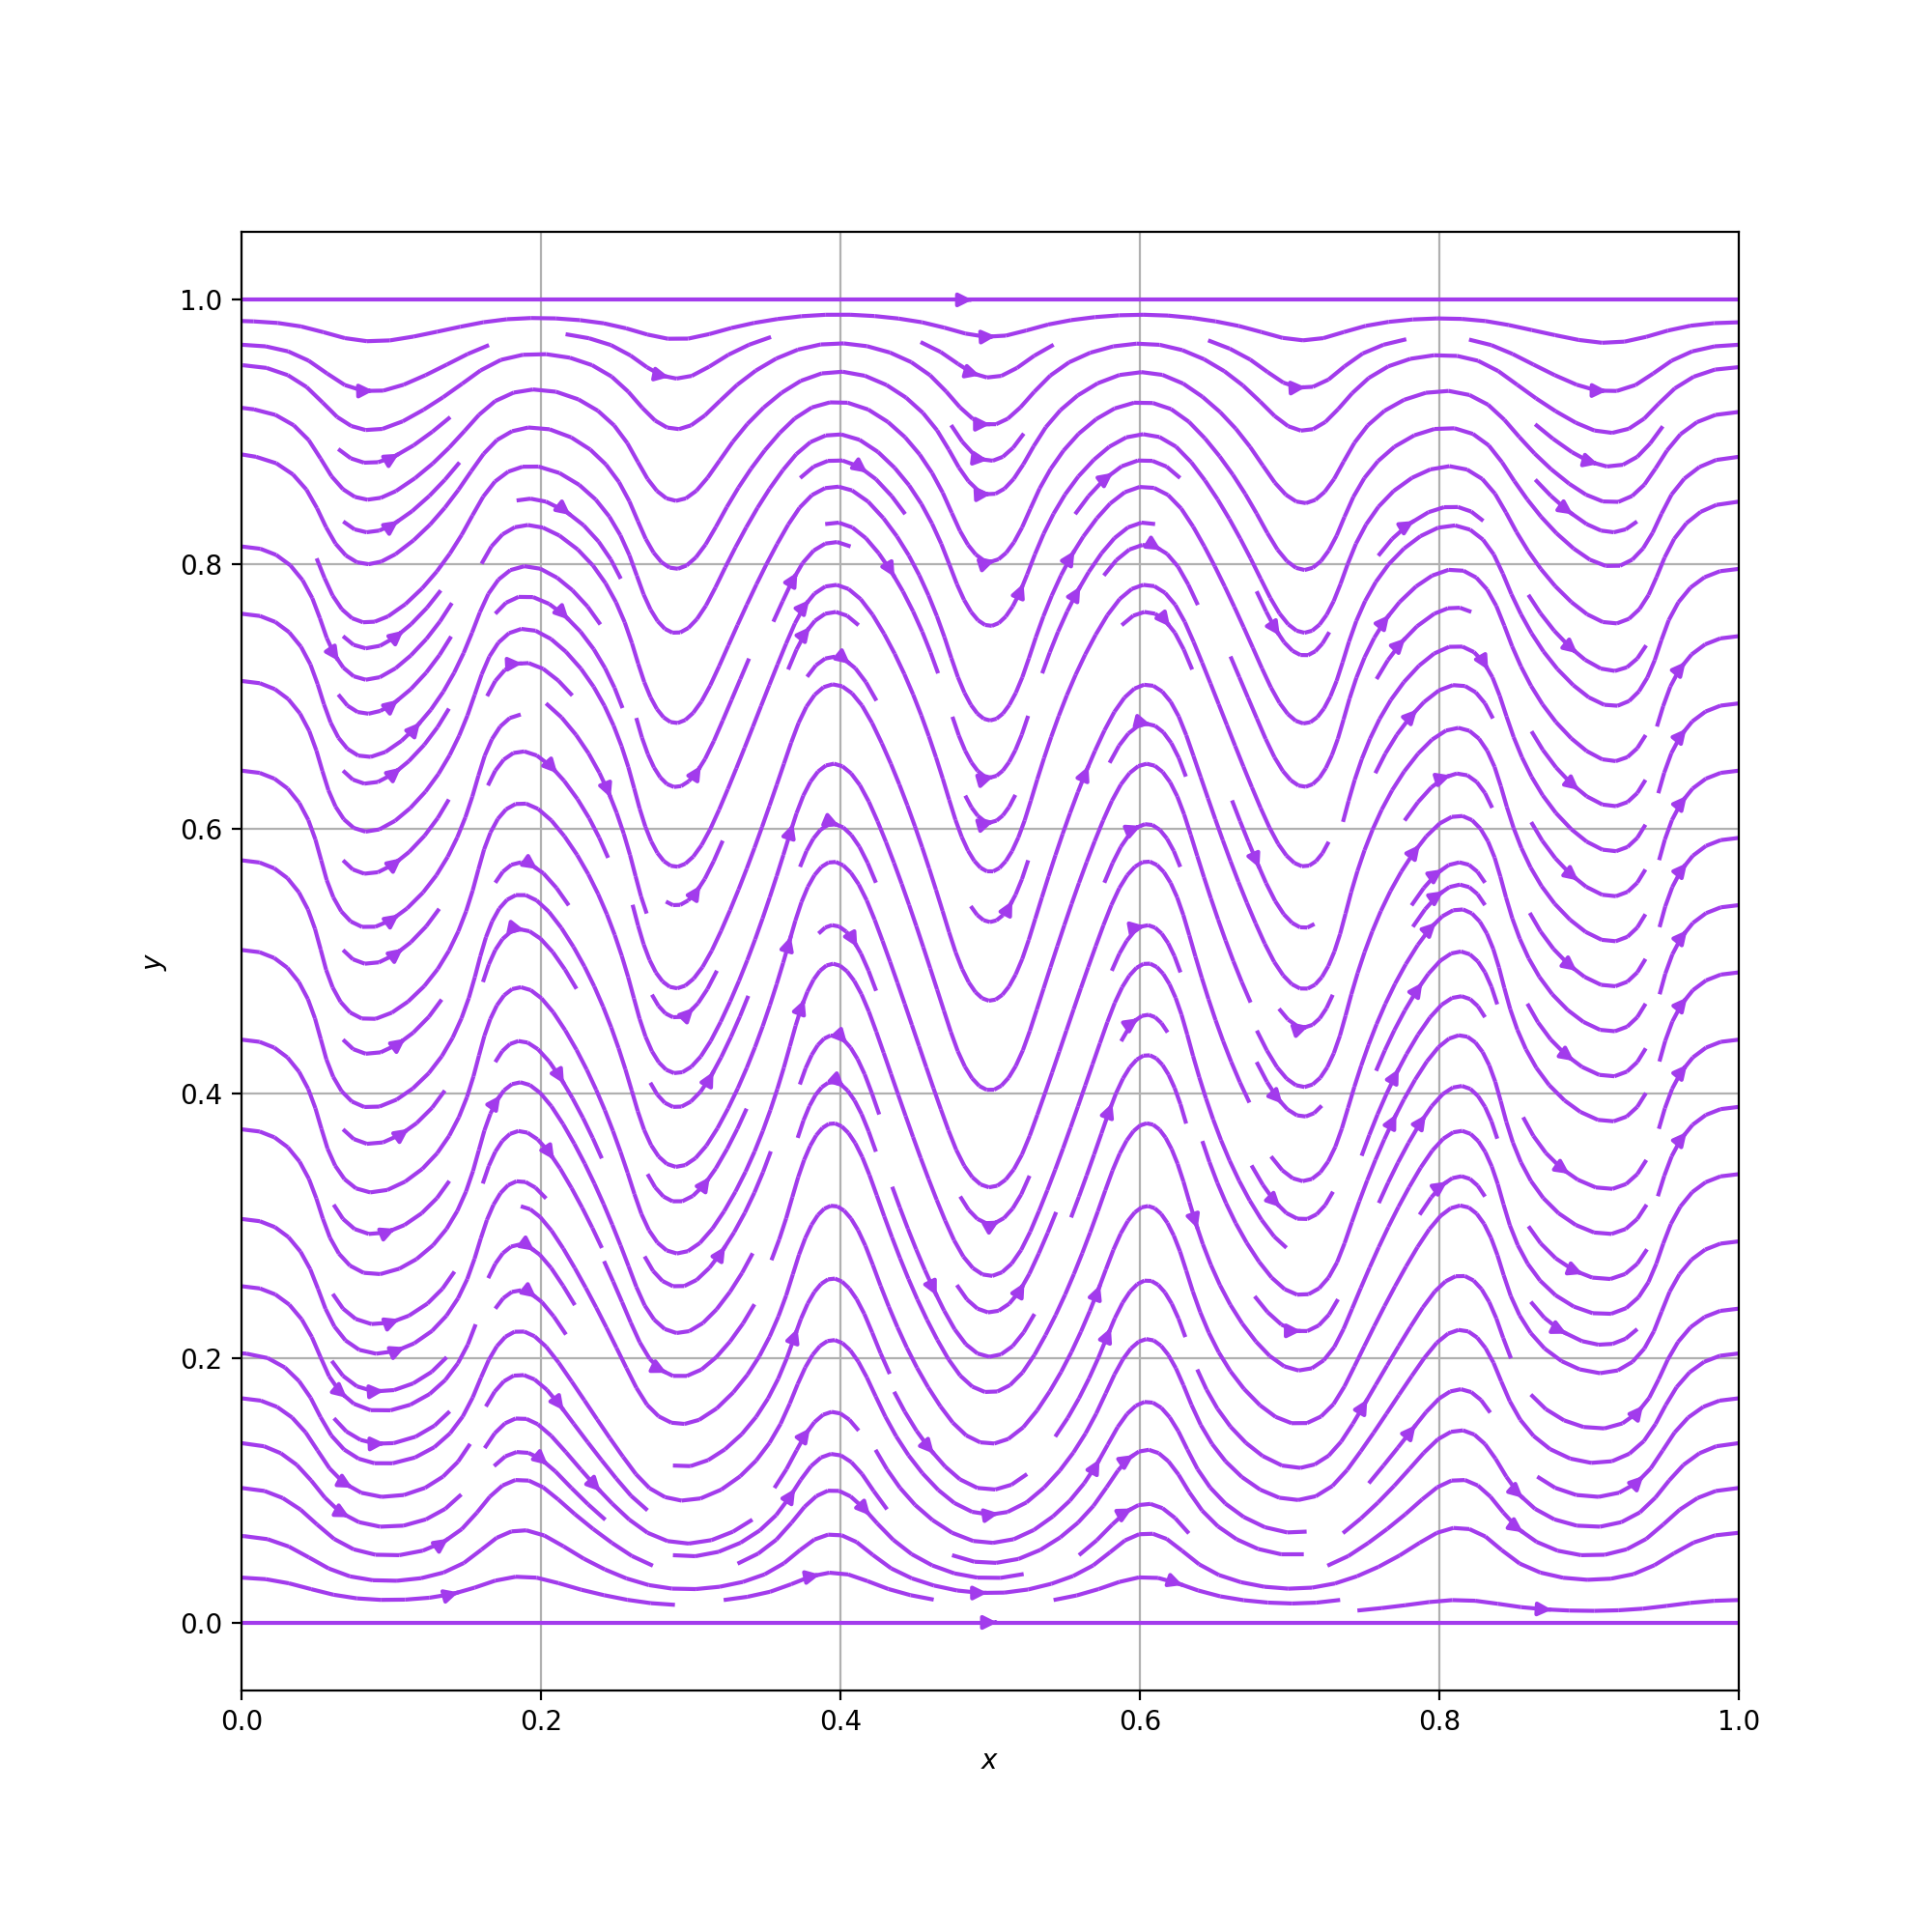
\includegraphics[width=\textwidth]{Pics/VectorField/E1b_a2_m10.png}
     \caption{$\alpha=2, m=10$}
 \end{subfigure}
 \caption{Electromagetic vector field $\mathbf{b}$ from (\ref{E1_b})} \label{E1_VFs}
\end{figure}
nice pictures with vector field
calculation of clossed field line
have vector field of 3 examples (3)
have f and the exact solution at different eps (12)

\subsection{Example 1, Numerical Demostration}
Show error plots for example for ranging eps  L and H (6)
Use MMAP, AP, Limit, SP, PF
Due to MMAP better than AP not use AP
Show stabalisation gives same MMAP and Stab
Do DN plot (1)
Changing grid size table 
size | dof | L2 error | H1 error PF, MMAP
Show gamma in can be on any part of streamline

\section{Example 2}
We now propose an example on an annulus with closed field lines.
We will solve the PDE (\ref{}) with $\Omega := \{x,y \in \mathbb{R}, 1<x^2+y^2<4\}$, $\Gamma_D := \{x,y \in \mathbb{R}, (x^2+y^2=1 \text{ or } x^2+y^2=4)\}$ and $\Gamma_N := \emptyset$. We chose the magnetic field 
\begin{equation}
\mathbf{b} = \frac{\mathbf{B}}{|\mathbf{B}|} = 
\left[ \begin{matrix}
-y\\
 x
\end{matrix} \right]/\sqrt{x^2+y^2}, 
\mathbf{B} = \left[ \begin{matrix}
-y\\
 x
\end{matrix} \right]
\end{equation}
We will use solution
\begin{equation}
u = (1+\varepsilon)(x^2 + y^2 -1)(4-x^2-y^2)
\end{equation}
From Fig \ref{} it can be seen the magnetic field have closed lines. Therefore, for methods which involve $\Gamma_{in}$ we use the stabilisation variants. However, from the numerical investigation of Example 1 we found that we can change $\Gamma_{in}$ to $\Gamma_{out}$ and get similar error. This strongly suggests that $\Gamma_{in}$ can represent a point on each streamline. Thus we will numerically investigate the consequence of setting $\Gamma_{in}:=\{x,y \in \mathbb{R}, x>0, y=0\}$.




Therefore, these results strongly suggests that we can apply the condition  will investigate the numerical solution when $\Gamma_{in}$ is applied to part of the streamline, as in the numerical

Do u and f plot for different eps (4)
Show error plots for example for ranging eps  L and H (6)
Use MMAP, Limit, SP, PF
Redo with stab variants (6)
Show stabalisation gives different MMAP and Stab and streamline
Do DN plot (1)

\section{Example 3, Magnetic Islands}
We now solve an example on a square domain with non-zero boundary conditions on $\Gamma_D$ and with closed and open field lines.
We will solve the PDE (\ref{}) with $\Omega = [0,1]^2, \Gamma_D = \{y=0 \text{ or } y=1\}$ and $\Gamma_N = \{x=0 \text{ or } x=1\}$. We chose a magnetic field such 
\begin{equation}
\mathbf{b} = \frac{\mathbf{B}}{|\mathbf{B}|}, 
\mathbf{B} = \left[ \begin{matrix}
-\cos(\pi y)\\
4a \sin(4 \pi x)
\end{matrix} \right]
\end{equation}
We will use exact solution
\begin{equation}
u = \sin(10\sin(\pi y)-10a\cos(4 \pi x)) + \varepsilon \cos(2 \pi x)\sin(10 \pi y)
\end{equation}
Do u and f plot for different eps (4)
Use MMAP, Limit, SP, PF
with stab variants (6)
Do DN plot (1)
Changing grid size table 
size | dof | L2 error | H1 error PF, MMAP

\section{Example 4, Magnetic Islands}
Why do an example with zero BC ?
We now introduce an example on a unit square where $\Gamma_D$ has zero boundary conditions. Additionally, this has open and closed field lines.
Thus on $\Omega = [0,1]^2, \Gamma_D = \{y=0 \text{ or } y=1\}$ and $\Gamma_N = \{x=0 \text{ or } x=1\}$ we solve the PDE (\ref{}) with the same magnetic
\begin{equation}
\mathbf{b} = \frac{\mathbf{B}}{|\mathbf{B}|}, 
\mathbf{B} = \left[ \begin{matrix}
-\cos(\pi y)\\
4a \sin(4 \pi x) \sin(\pi y)
\end{matrix} \right]
\end{equation}
Where the exact solution is 
\begin{equation}
u = \sin(10 \sin(\pi y) \exp^{-a\cos(4 \pi x)}) 
\end{equation}
Do u and f plot for different eps (4)
Use MMAP, Limit, SP, PF
with stab variants (6)
Do DN plot (1)
Changing grid size table 
size | dof | L2 error | H1 error PF, MMAP

\section{Example 5, Torus}
We now look at an example in 3D where the domain $\Omega $ is a torus with inner radius $r_I = 1$, outer radius $r_O = 0.5$ and is centred at the origin. It will have zero Dirichlet boundary conditions. For this eaxmple we will use Toroidal coordinates which are explained in Appendix \ref{} and demonstrate how to find the inverse map. We invert back to cartesian cordinates because the toroidal laplacian \cite{} is very complicated. Thus the definition of $r$ is
\begin{equation}
r = \sqrt{r_I^2 + x^2 + y^2 + z^2 -2r_I\sqrt{x^2+y^2}}
\end{equation}
Where $r$ denotes the minimum distance from the circulfurance of a circle centered at the origin with radius $r_I$ and has $z=0$. We have magnetic field 
\begin{equation}
\mathbf{b} = \frac{\mathbf{B}}{|\mathbf{B}|} = 
\left[ \begin{matrix}
-y\\
 x \\
 0
\end{matrix} \right]/\sqrt{x^2+y^2}, 
\mathbf{B} = \left[ \begin{matrix}
-y\\
 x\\
 0
\end{matrix} \right]
\end{equation}
Also, we will have exact solution
\begin{equation}
u = 
\begin{cases}
(1+\varepsilon)((0.5)^2 - r ),\\
(1+\varepsilon)(0.25 -  \sqrt{r_I^2 + x^2 + y^2 + z^2 -2r_I\sqrt{x^2+y^2}})
\end{cases}
\end{equation}
do u anf f but only for eps -10
Use MMAP, Limit, SP, PF
with stab variants (6)
\section{Methods For Investigation}

\subsection{Line Integration}


\subsection{Mapping of f}


\subsection{Splitting of domain}

\printbibliography[heading=bibintoc]

\appendix

\section{Title of Appendix}

Appendices are definitely not necessary and assessors are not obliged to read them so only use them for non-vital text, figures or calculations.$\phi$

\subsection{Toroidal Coordinates}
Here we discuss how to parameterise a torus and to find its inverted map. We use the Figures \ref{Torus_XY} and \ref{Torus_z} below to help us derive the parameterisation.
\begin{figure}[H]
 \begin{subfigure}{0.5\textwidth}
     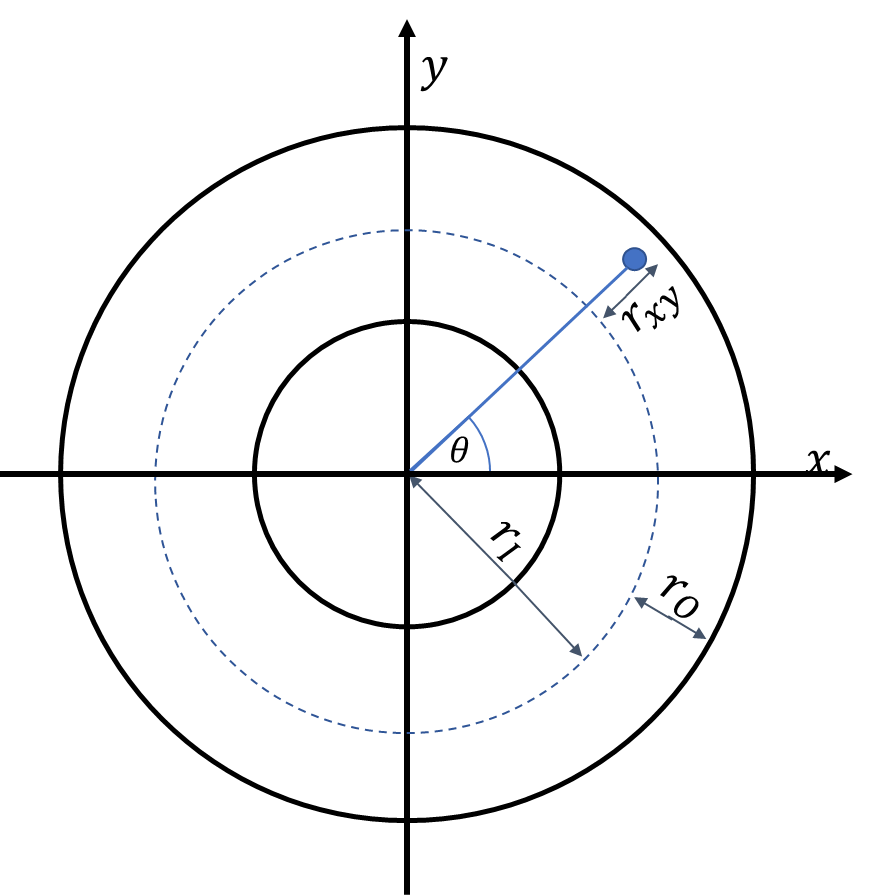
\includegraphics[width=\textwidth]{Pics/TorusCordsXY.png}
     \caption{Cross section of torus with $z=0$}
     \label{Torus_XY}
 \end{subfigure}
 \hfill
 \begin{subfigure}{0.5\textwidth}
     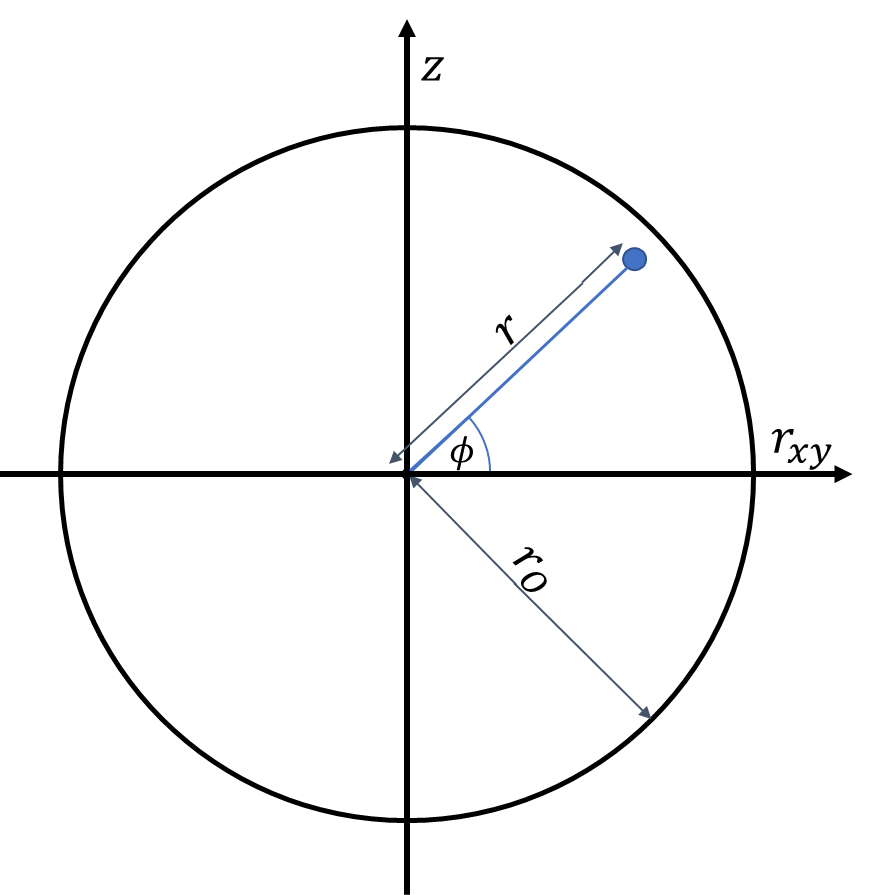
\includegraphics[width=\textwidth]{Pics/TorusCordsr_XYZ.png}
     \caption{Cross section of torus}
     \label{Torus_z}
 \end{subfigure}
 \caption{Visual aids for the derivation of the Toroidal parameterisation.} \label{BO}
\end{figure}

From visual inspection of Figure \ref{Torus_XY} we get 
\begin{align}
x &= (r_I + r_{xy})\cos(\theta)\\
y &= (r_I + r_{xy})\sin(\theta)
\end{align}
Additionally, from Figure \ref{Torus_z} we get 
\begin{align}
r_{xy}& = r \cos(\phi) \\
z &= r \sin(\phi)
\end{align}
Thus joining the equations (\ref{}) to (\ref{}) we get the toroidal parametrisation
\begin{align}
x &= (r_I + r\cos(\phi))\cos(\theta) \\
y &= (r_I + r \cos(\phi))\sin(\theta) \\
z &= r \sin(\phi)
\end{align}
where $0\leq r \leq r_O$ and $0 \leq \phi, \theta \leq 2 \pi$. Now we calculate the inverse of this map by considering $x^2 + y^2 + z^2$. 
\begin{align}
x^2 + y^2 + z^2 &= (r_I + r \cos(\phi))^2 + r^2\sin^2(\phi)\\
&= r_I^2 + 2r_Ir\cos(\phi) + r^2\\
&= r_I^2 +2r_I \sqrt{r^2-z^2} + r^2
\end{align}
This is a quadratic in disguise thus after some algebraic manipulation we get $4$ possible solutions
\begin{equation}
r = \pm\sqrt{r_I^2 + x^2 + y^2 + z^2 \pm 2r_I\sqrt{x^2+y^2}}
\end{equation}
However, by using enforcing $r\geq0$ we remove two solutions. We find the final solution by substitution. We use the substitution $(x, y, z) = (r_I, 0, 0)$ where $r=0$. With $+$ we get $r=2r_I$ and for $-$ we get $r = 0$. Thus we have 
\begin{equation}
r = \sqrt{r_I^2 + x^2 + y^2 + z^2 - 2r_I\sqrt{x^2+y^2}}
\end{equation}
For completeness will we calculate $\theta$ and $\phi$. To get $\theta$ and $\phi$ we do a similar process used for calculating the argument of complex numbers. We note $r_{xy}=x^2+y^2-r_I$ thus we get
\begin{align}
\theta &= \text{atan2}(y, x) \\
\phi &= \text{atan2}(z, x^2+y^2-r_{I})
\end{align}
where atan2 is a common variation of the arctan function.

We use the inverse of the map because calculating the differential operators leads to large expressions. These expressions can be found in \cite{}. When we need to solve a PDE on a domain which can be parameterised it is usually easier to turn the source term $f$ into Cartesian coordinates so we deal with the Cartesian differential operators.

\subsection{Formulation of examples}
How i found the exact solution for problems 
\section{CG Order 2}
In our numerical simulations we use a continuous Lagrange order $2$ finite element. We now provide a method for the derivation of this finite element on an interval and a triangle. Additionally, following a similar procedure we can derive the basis functions for other domains. The resource \cite{} states basis functions for many finite elements.This is not implemented in code we instead use the Firedrake implementation of CG order $2$. 

For each element we have basis functions $\phi_i(\mathbf{x})$ which have a linear combination from the set $\{1, x, x^2, y, y^2, z, z^2, xy, yz, xz\}$ and locations on domain $\ell_i$.  To find the coefficients of the linear combination we must solve
\begin{equation} \label{CG_eq}
\phi_i(\ell_j) =
\begin{cases}
1, &i=j,\\
0, &i\neq j.
\end{cases}
\end{equation}
It should be noted we can do a substitution to make the shapes unit size.
\subsection{Interval (1D)}
Therefore, we have $i \in \{0, 1, 2\}$ and basis functions 
\begin{equation}
\phi_i(x) = \xi_{i0} + \xi_{i1}x + \xi_{i2}x^2
\end{equation}
with $\ell_0 = 0, \ell_1 = 1$ and $\ell_2 = 0.5$. Thus by using (\ref{CG_eq}) we get equations to solve
\begin{align}
\phi_i(\ell_0) = \phi_i(0) &= \xi_{i0} &= \delta_{i0},\\
\phi_i(\ell_1) = \phi_i(1) &= \xi_{i0} + \xi_{i1} + \xi_{i2} &= \delta_{i1},\\
\phi_i(\ell_2) = \phi_i(0.5) &= \xi_{i0} + \frac{\xi_{i1}}{2} + \frac{\xi_{i2}}{4} &= \delta_{i2}
\end{align}
where $\delta$ represents Kronecker delta. This can be put into matrix form
\begin{equation}
\left[ \begin{matrix}
\xi_{i0} & \xi_{i1} & \xi_{i2}
\end{matrix} \right]
\left[ \begin{matrix}
1 & 1 & 1 \\
0 & 1 & 1/2 \\
0 & 1 & 1/4
\end{matrix} \right] = 
\left[ \begin{matrix}
\delta_{i0} & \delta_{i1} & \delta_{i2}
\end{matrix} \right]
\end{equation}
It is trivial to implement this into a matrix for all basis functions in this element.
\begin{equation}
\left[ \begin{matrix}
\xi_{00} & \xi_{01} & \xi_{02} \\
\xi_{10} & \xi_{11} & \xi_{12} \\
\xi_{20} & \xi_{21} & \xi_{22} 
\end{matrix} \right]
\left[ \begin{matrix}
1 & 1 & 1 \\
0 & 1 & 1/2 \\
0 & 1 & 1/4
\end{matrix} \right] = 
\left[ \begin{matrix}
1 & 0 & 0 \\
0 & 1 & 0 \\
0 & 0 & 1
\end{matrix} \right]
\end{equation}
Thus we get 
\begin{align}
\left[ \begin{matrix}
\xi_{00} & \xi_{01} & \xi_{02} \\
\xi_{10} & \xi_{11} & \xi_{12} \\
\xi_{20} & \xi_{21} & \xi_{22} 
\end{matrix} \right] &= 
\left[ \begin{matrix}
1 & 1 & 1 \\
0 & 1 & 1/2 \\
0 & 1 & 1/4
\end{matrix} \right]^{-1}, \\
\left[ \begin{matrix}
\xi_{00} & \xi_{01} & \xi_{02} \\
\xi_{10} & \xi_{11} & \xi_{12} \\
\xi_{20} & \xi_{21} & \xi_{22} 
\end{matrix} \right] &= 
\left[ \begin{matrix}
1 & -3 & 2 \\
0 & -1 & 2 \\
0 & 4 & -4
\end{matrix} \right],
\end{align}
This leads to the basis functions
\begin{align}
\phi_0(x) &= 2x^2-3x+1,\\
\phi_1(x) &= x(2x-1),\\
\phi_2(x) &= 4x(1-x)
\end{align}
With there visual representation in Figure \ref{InterFuncs}.
\begin{figure}[H]
     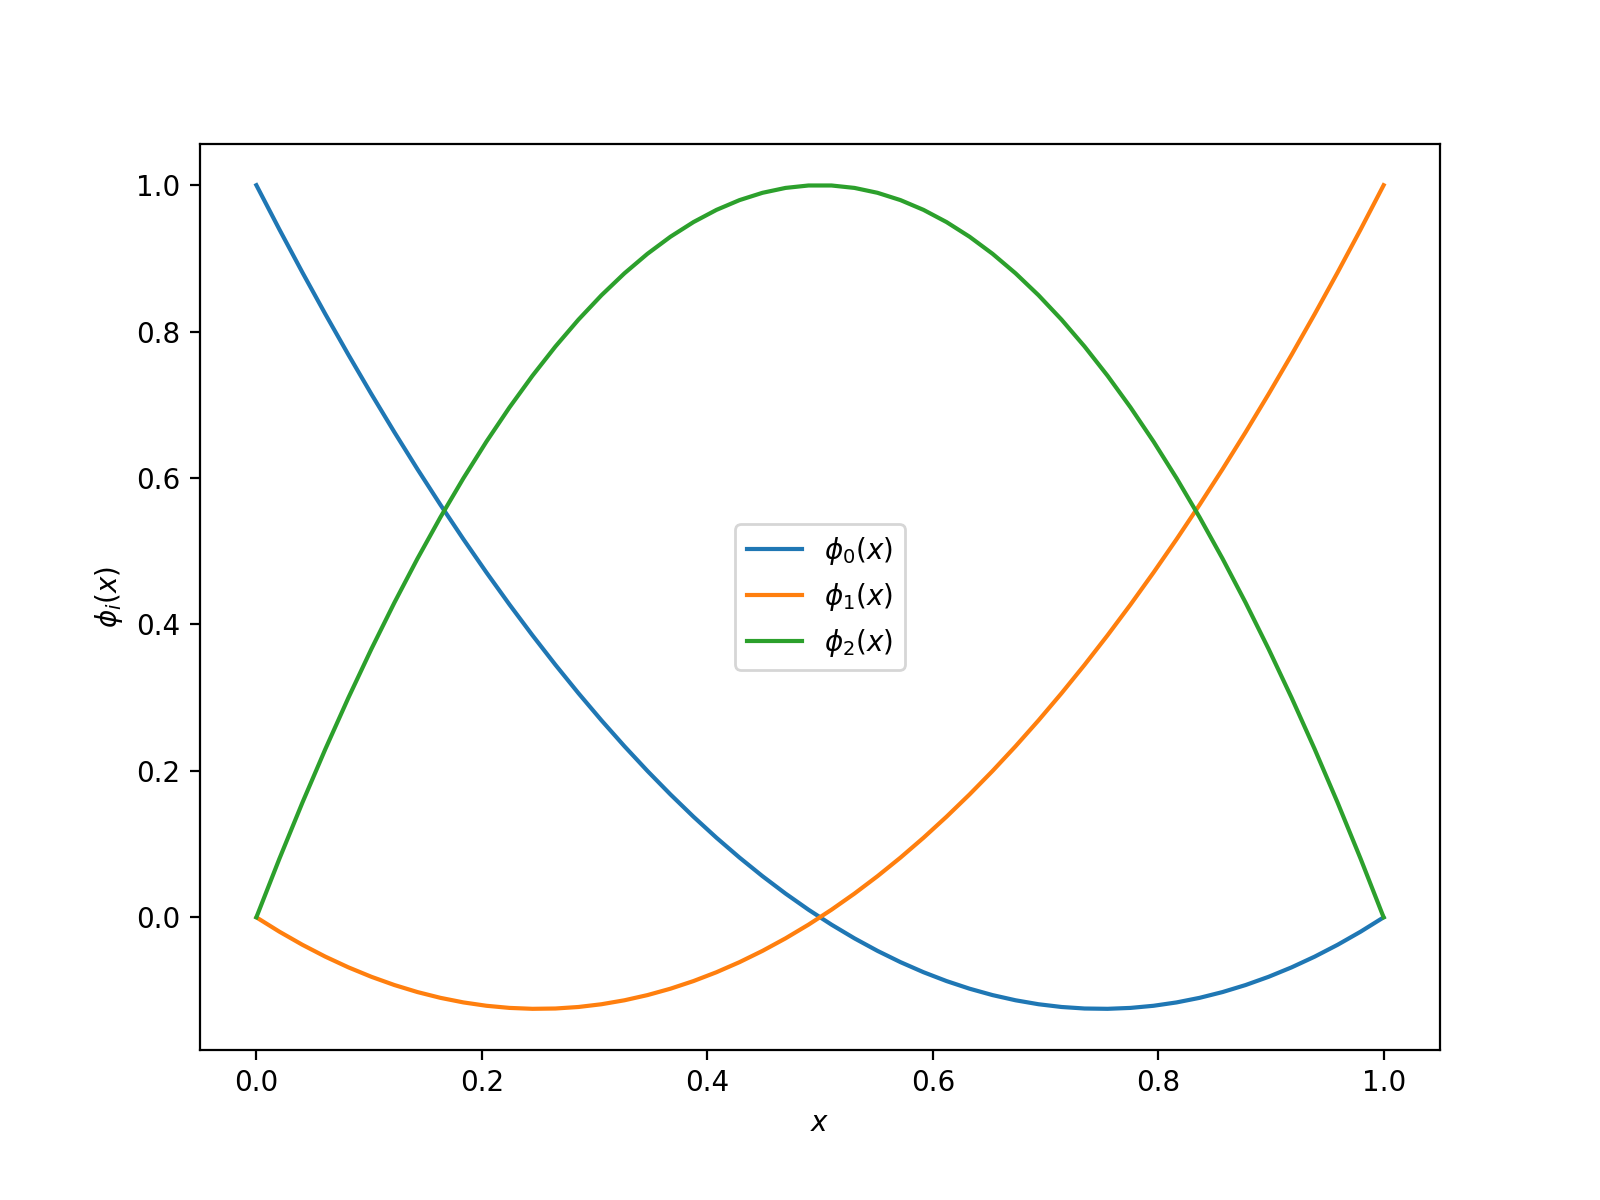
\includegraphics[width=\textwidth]{Pics/BasisFunc/IntervalFuncs.png}
     \caption{Lagrage order 2 basis functions  on interval $[0,1]$}
     \label{InterFuncs}
\end{figure}

\subsection{Triangle (2D)}
For an order $2$ Lagrange element on a triangle we have $i \in \{0, 1, 2,3,4,5\}$ and the basis functions are of the form
\begin{equation}
\phi_i(x,y) = \xi_{i0} + \xi_{i1} x + \xi_{i2} y + \xi_{i3} xy + \xi_{i4} x^2 + \xi_{i5}y^2,
\end{equation}
where the domain is $x+y\leq 1, x \geq 0$ and $y\geq 0$. For $\ell_i$ we get
\begin{align}
\ell_0 &= (0,0), &\ell_3 = (1/2,1/2), \\
\ell_1 &= (1,0), &\ell_4 = (0,1/2), \\
\ell_2 &= (0,1), &\ell_5 = (1/2,0),
\end{align}
This leads to the set of equations
\begin{align}
\phi_i(\ell_0) &= \xi_{i0}, \\
\phi_i(\ell_1) &= \xi_{i0} + \xi_{i1} + \xi_{i4}, \\
\phi_i(\ell_2) &= \xi_{i0} + \xi_{i2} + \xi_{i5}, \\
\phi_i(\ell_3) &= \xi_{i0} + \frac{\xi_{i1}+\xi_{i2}}{2} + \frac{\xi_{i3} + \xi_{i4} + \xi_{i5}}{4}, \\
\phi_i(\ell_4) &= \xi_{i0} + \frac{\xi_{i2}}{2} + \frac{\xi_{i5}}{4}, \\
\phi_i(\ell_5) &= \xi_{i0} + \frac{\xi_{i1}}{2} + \frac{\xi_{i4}}{4},
\end{align}
Therefore, using the equations created by (\ref{CG_eq}) we get the matrix of coficeits
\begin{align}
\left[ \begin{matrix}
\xi_{00} & \xi_{01} & \xi_{02} & \xi_{03} & \xi_{04} & \xi_{05}\\
\xi_{10} & \xi_{11} & \xi_{12} & \xi_{13} & \xi_{14} & \xi_{25}\\
\xi_{20} & \xi_{21} & \xi_{22} & \xi_{23} & \xi_{24} & \xi_{25}\\
\xi_{30} & \xi_{31} & \xi_{32} & \xi_{33} & \xi_{34} & \xi_{35}\\
\xi_{40} & \xi_{41} & \xi_{42} & \xi_{43} & \xi_{44} & \xi_{45}\\
\xi_{50} & \xi_{51} & \xi_{52} & \xi_{53} & \xi_{54} & \xi_{55}
\end{matrix} \right] &= 
\left[ \begin{matrix}
1 & 1 & 1 & 1 & 1 & 1\\
0 & 1 & 0 & 1/2 & 0 & 1/2\\
0 & 0 & 1 & 1/2 & 1/2 & 0\\
0 & 0 & 0 & 1/4 & 0 & 0\\
0 & 1 & 0 & 1/4 & 0 & 1/4\\
0 & 0 & 1 & 1/4 & 1/4 & 0
\end{matrix} \right]^{-1}, \\
\left[ \begin{matrix}
\xi_{00} & \xi_{01} & \xi_{02} & \xi_{03} & \xi_{04} & \xi_{05}\\
\xi_{10} & \xi_{11} & \xi_{12} & \xi_{13} & \xi_{14} & \xi_{25}\\
\xi_{20} & \xi_{21} & \xi_{22} & \xi_{23} & \xi_{24} & \xi_{25}\\
\xi_{30} & \xi_{31} & \xi_{32} & \xi_{33} & \xi_{34} & \xi_{35}\\
\xi_{40} & \xi_{41} & \xi_{42} & \xi_{43} & \xi_{44} & \xi_{45}\\
\xi_{50} & \xi_{51} & \xi_{52} & \xi_{53} & \xi_{54} & \xi_{55}
\end{matrix} \right] &= 
\left[ \begin{matrix}
1 & -3 & -3 & 4 & 2 & 2\\
0 & -1 & 0 & 0 & 2 & 0\\
0 & 0 & -1 & 0 & 0 & 2\\
0 & 0 & 0 & 4 & 0 & 0\\
0 & 0 & 4 & -4 & 0 & -4\\
0 & 4 & 0 & -4 & -4 & 0
\end{matrix} \right]
\end{align}
Thus leading to basis functions
\begin{align}
\phi_0(x,y) &= 2(x+y)^2 - 3(x+y) + 1, \\
\phi_1(x,y) &= x(2x-1), \\
\phi_2(x,y) &= y(2y-1), \\
\phi_3(x,y) &= 4xy, \\
\phi_4(x,y) &= 4y(1-x-y), \\
\phi_5(x,y) &= 4x(1-x-y),
\end{align}
With the visual representation in Figure \ref{triBasisFuncs}.
\begin{figure}[H]
 \begin{subfigure}{0.5\textwidth}
     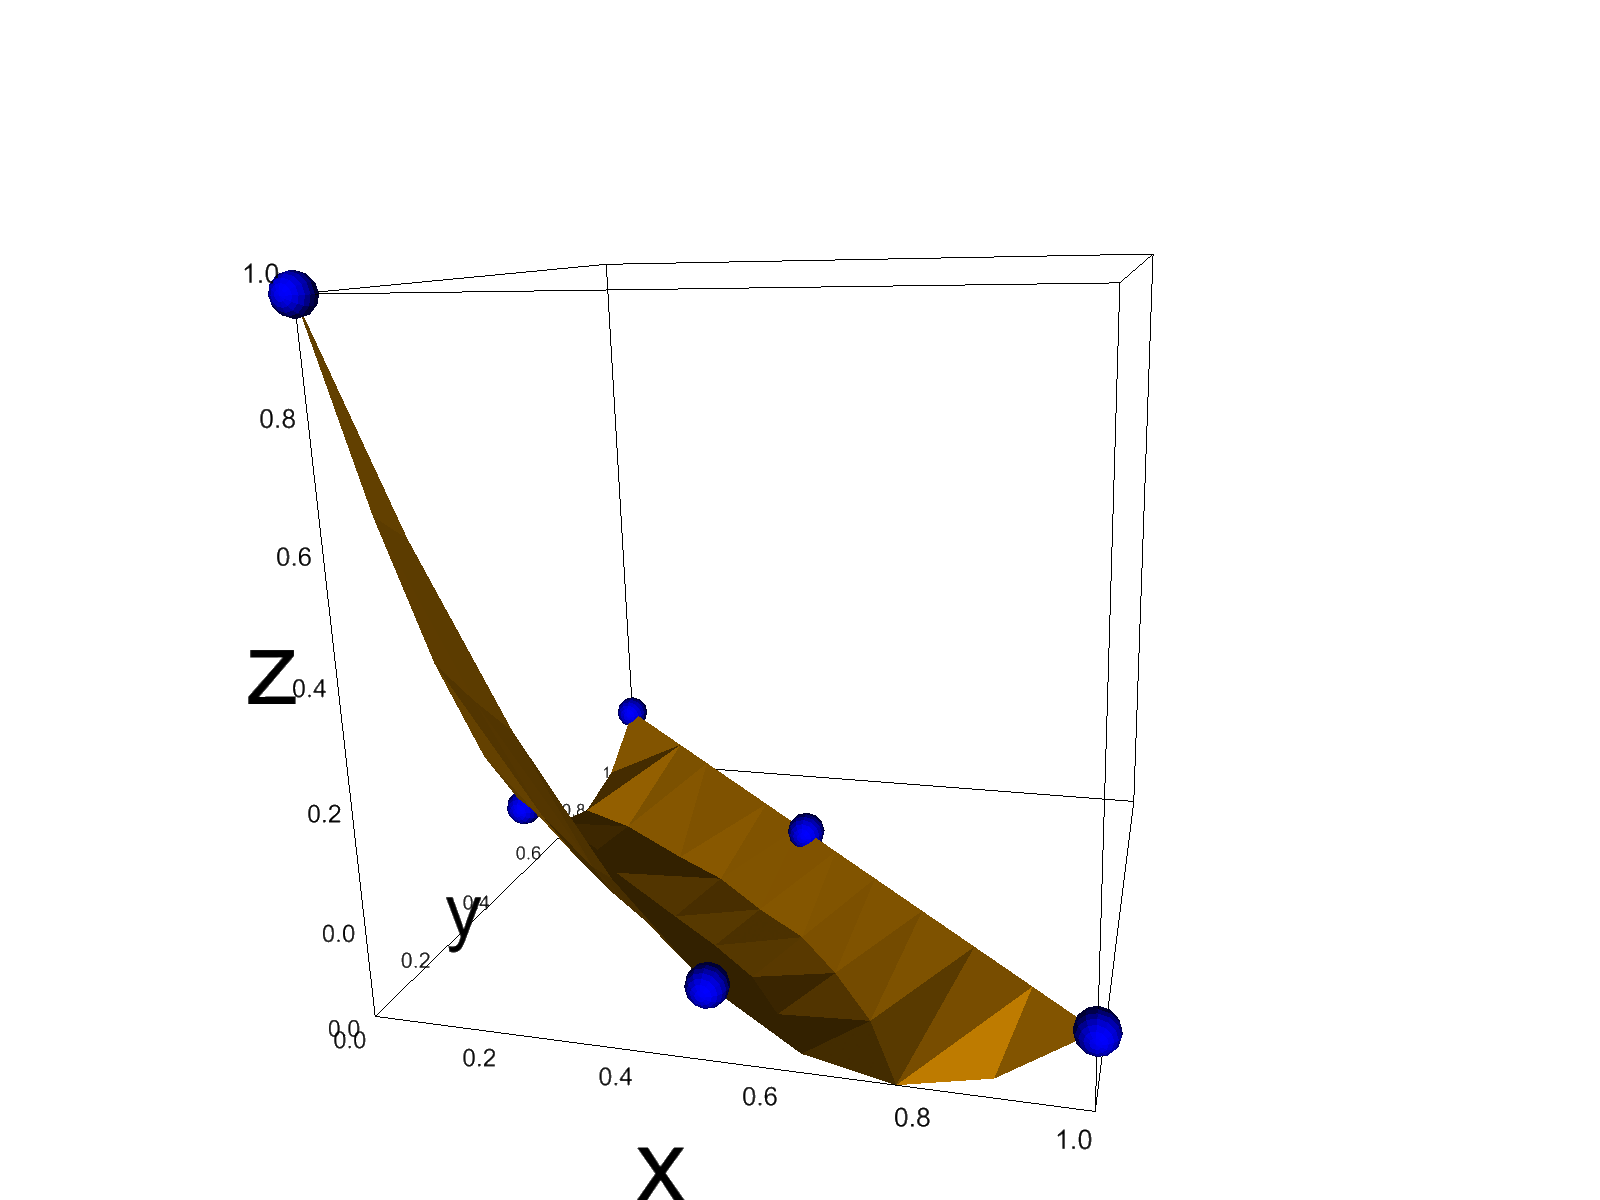
\includegraphics[width=\textwidth]{Pics/BasisFunc/triBasis0.png}
     \caption{\phi_0(x,y) = 2(x+y)^2 - 3(x+y) + 1,}
 \end{subfigure}
 \hfill
 \begin{subfigure}{0.5\textwidth}
     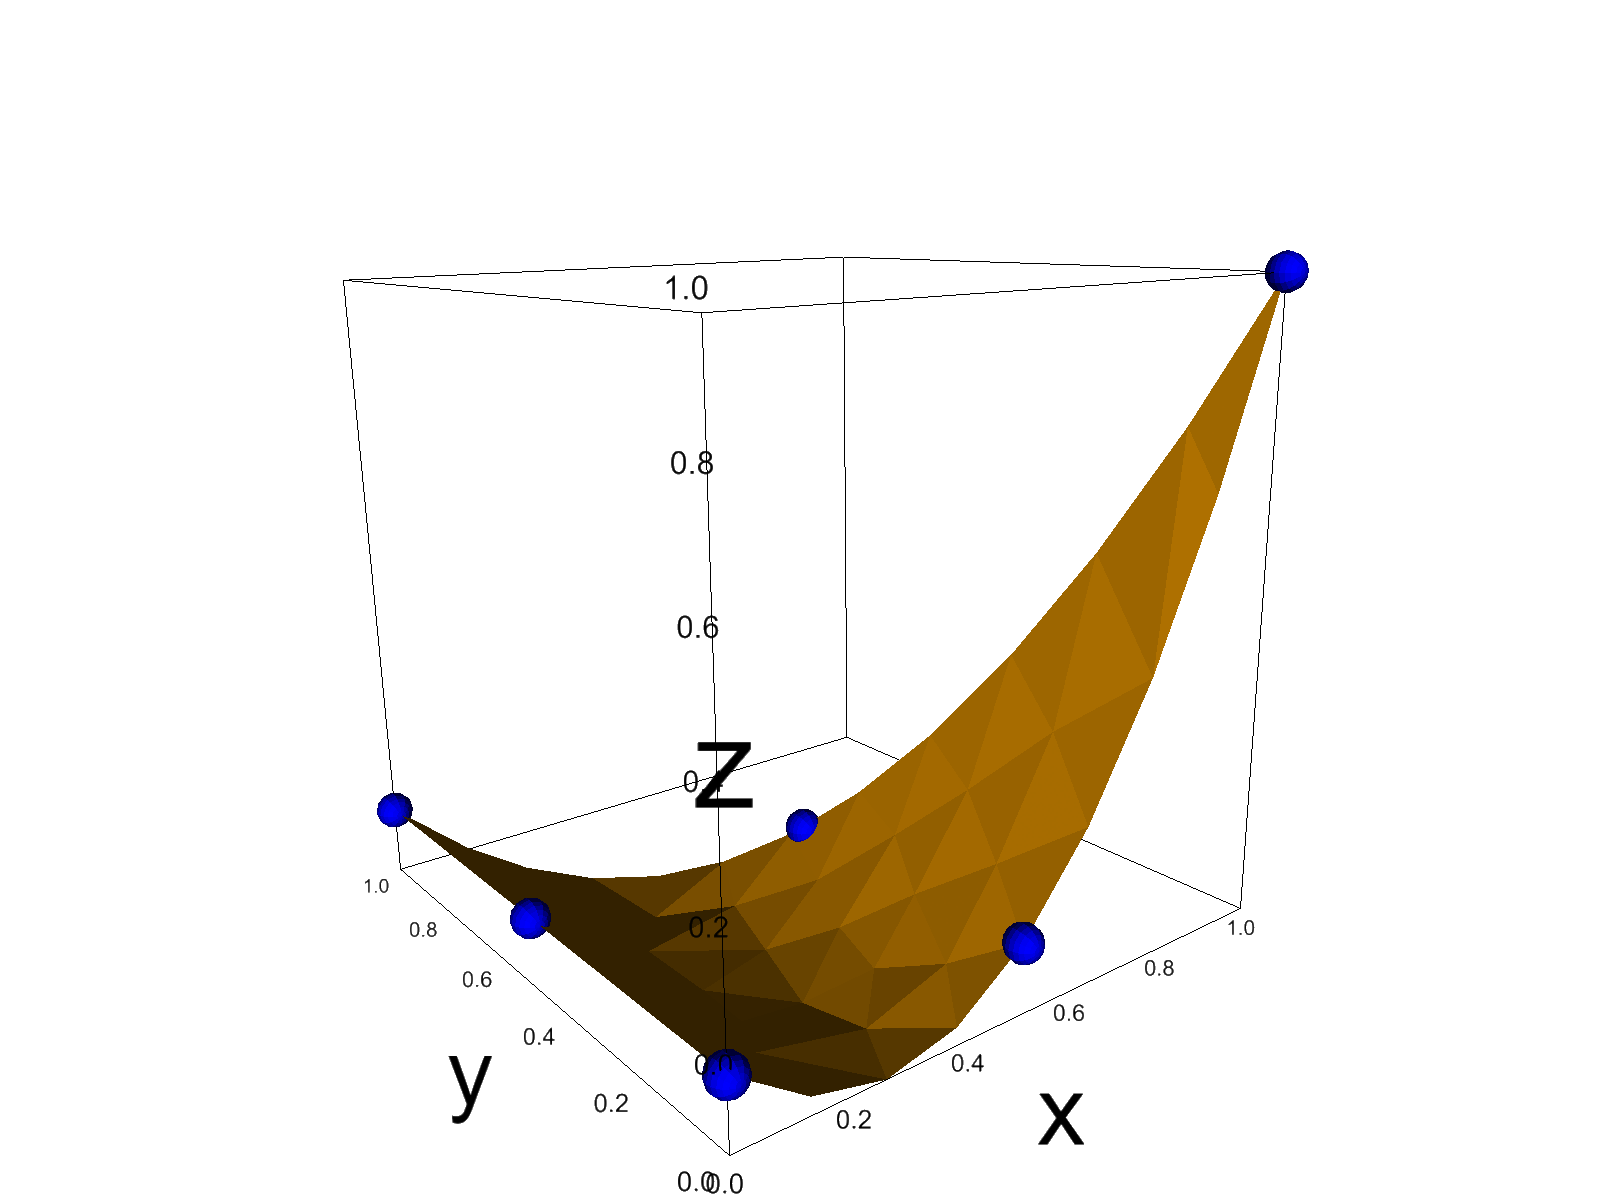
\includegraphics[width=\textwidth]{Pics/BasisFunc/triBasis1.png}
     \caption{\phi_1(x,y) = x(2x-1),}
 \end{subfigure}
 \hfill
 \begin{subfigure}{0.5\textwidth}
     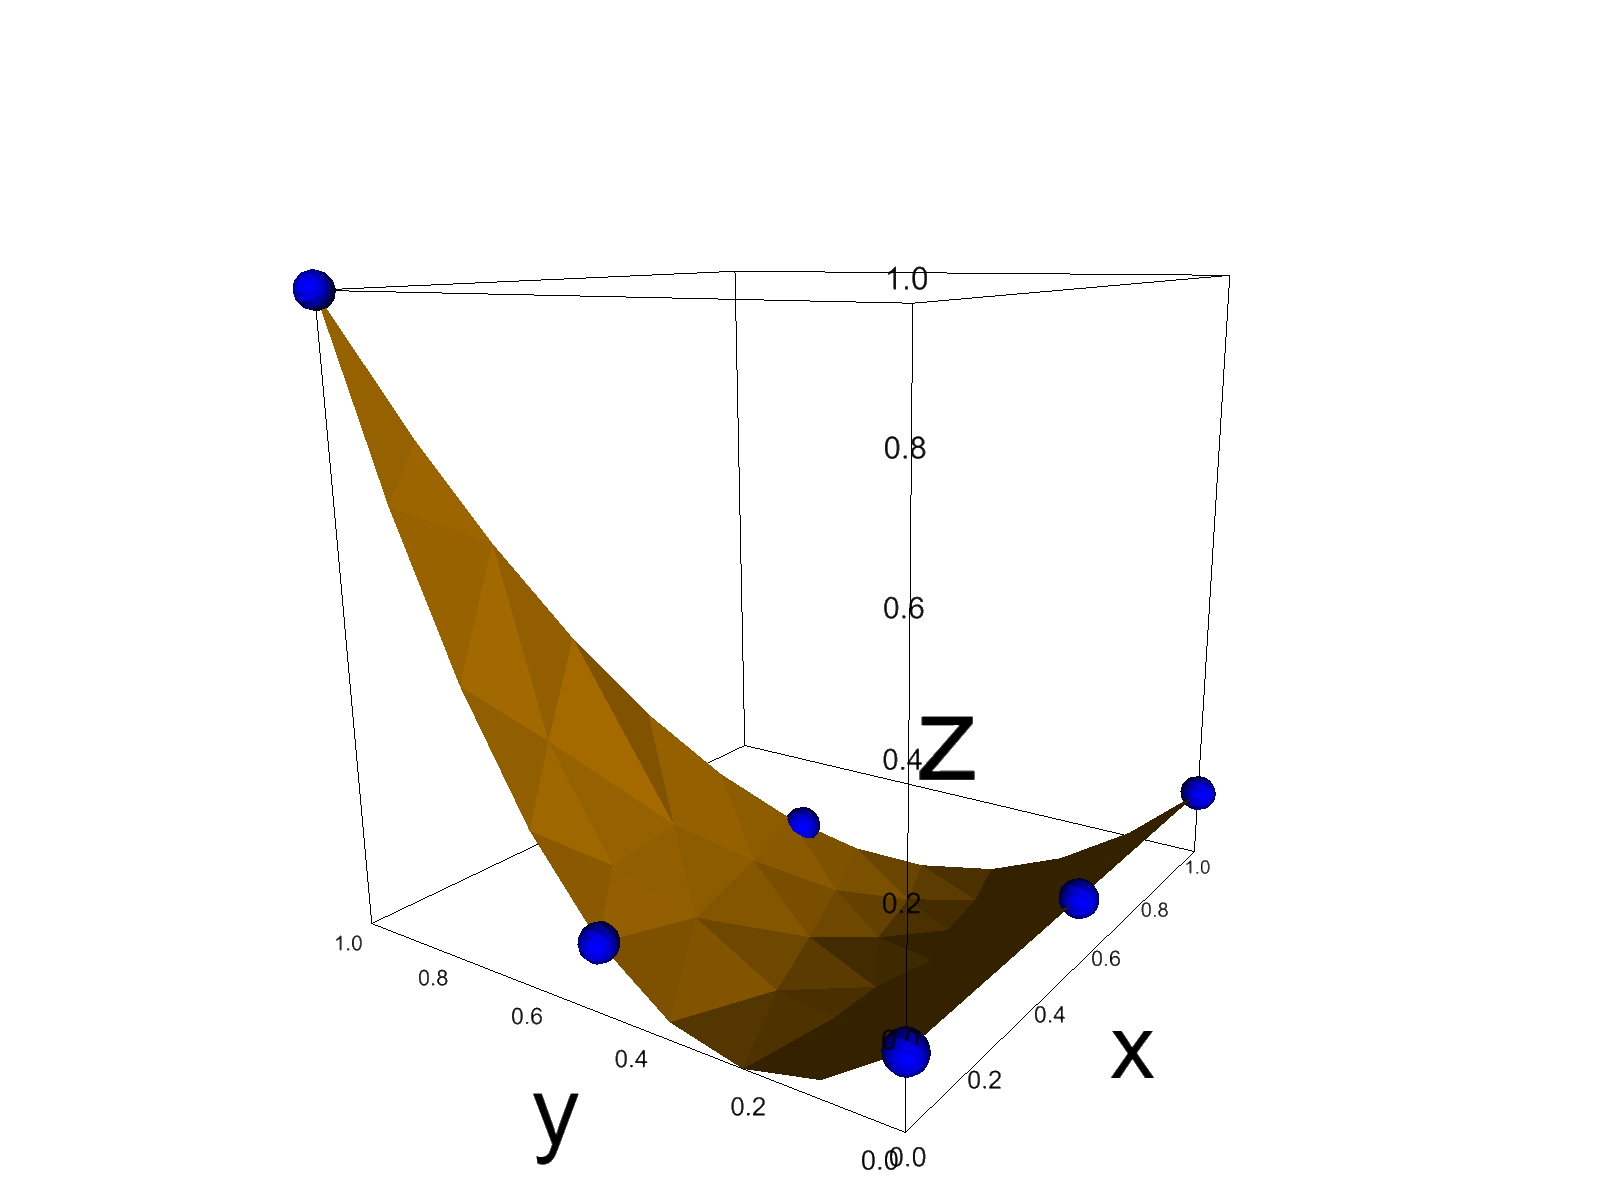
\includegraphics[width=\textwidth]{Pics/BasisFunc/triBasis2.png}
     \caption{\phi_2(x,y) = y(2y-1),}
 \end{subfigure}
 \hfill
 \begin{subfigure}{0.5\textwidth}
     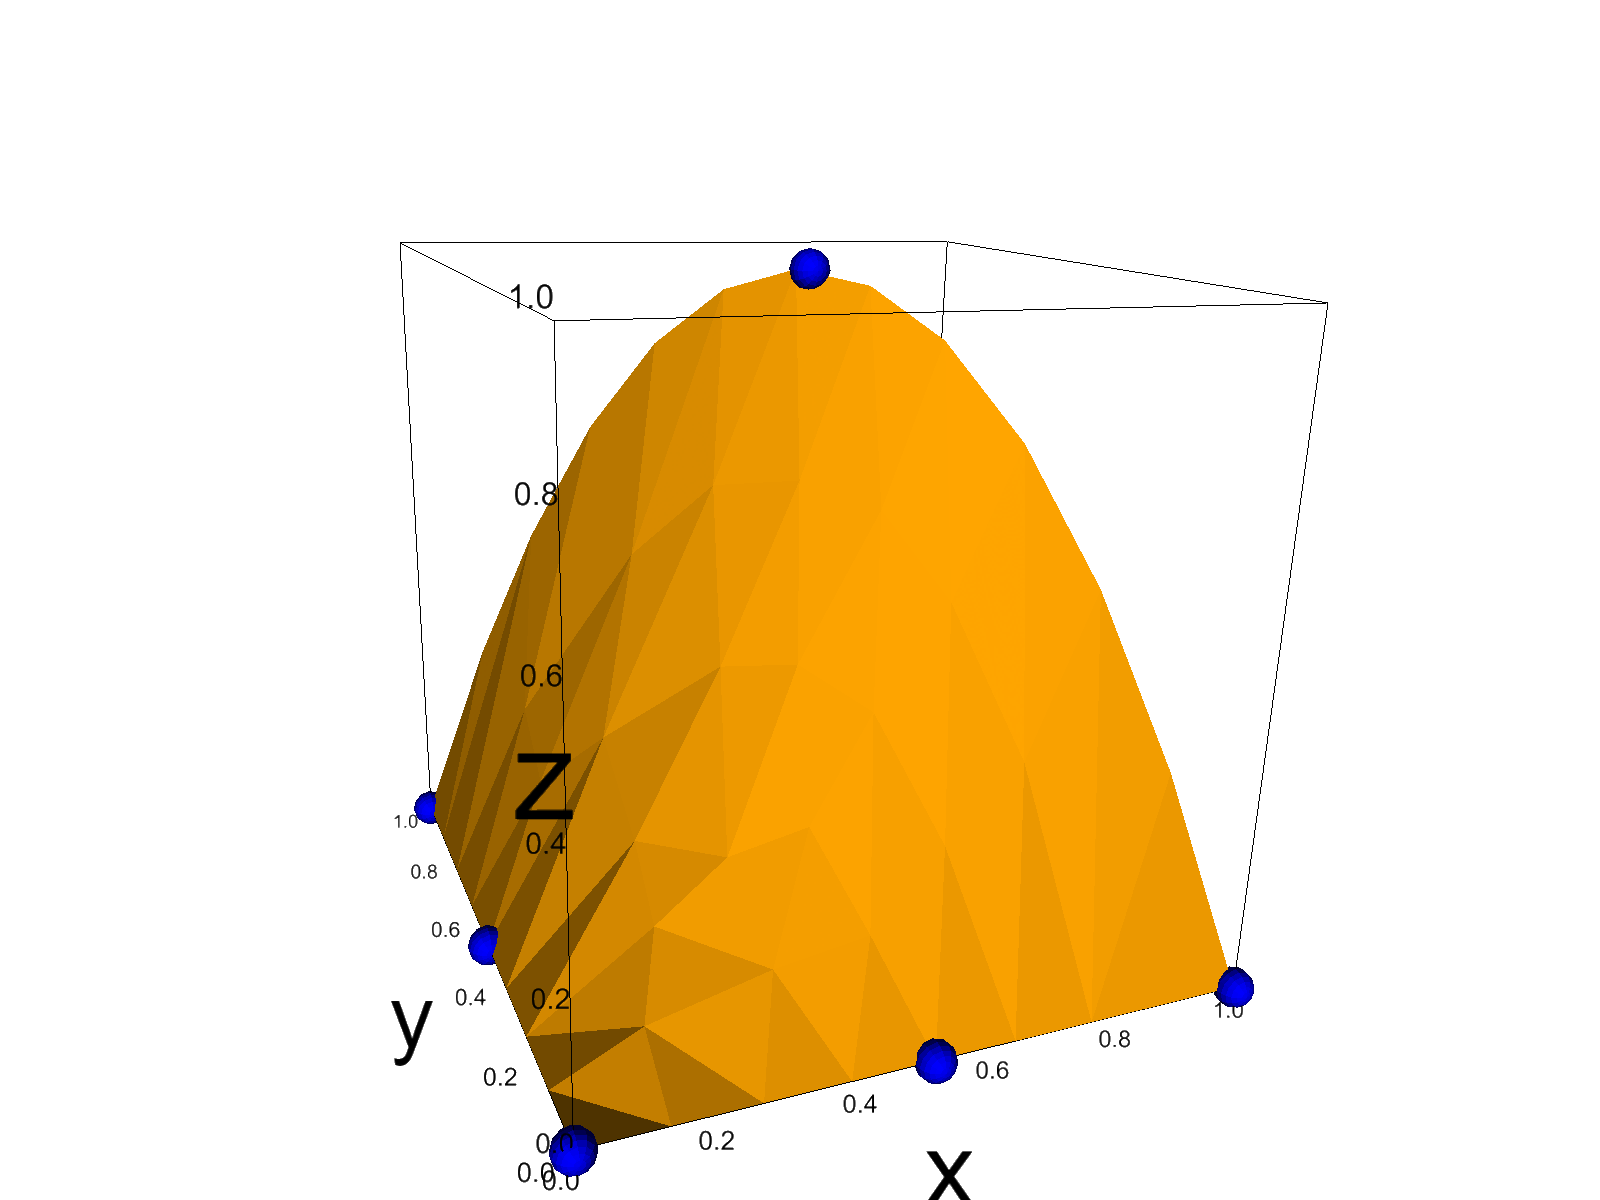
\includegraphics[width=\textwidth]{Pics/BasisFunc/triBasis3.png}
     \caption{\phi_3(x,y) = 4xy,}
 \end{subfigure}
 \hfill
 \begin{subfigure}{0.5\textwidth}
     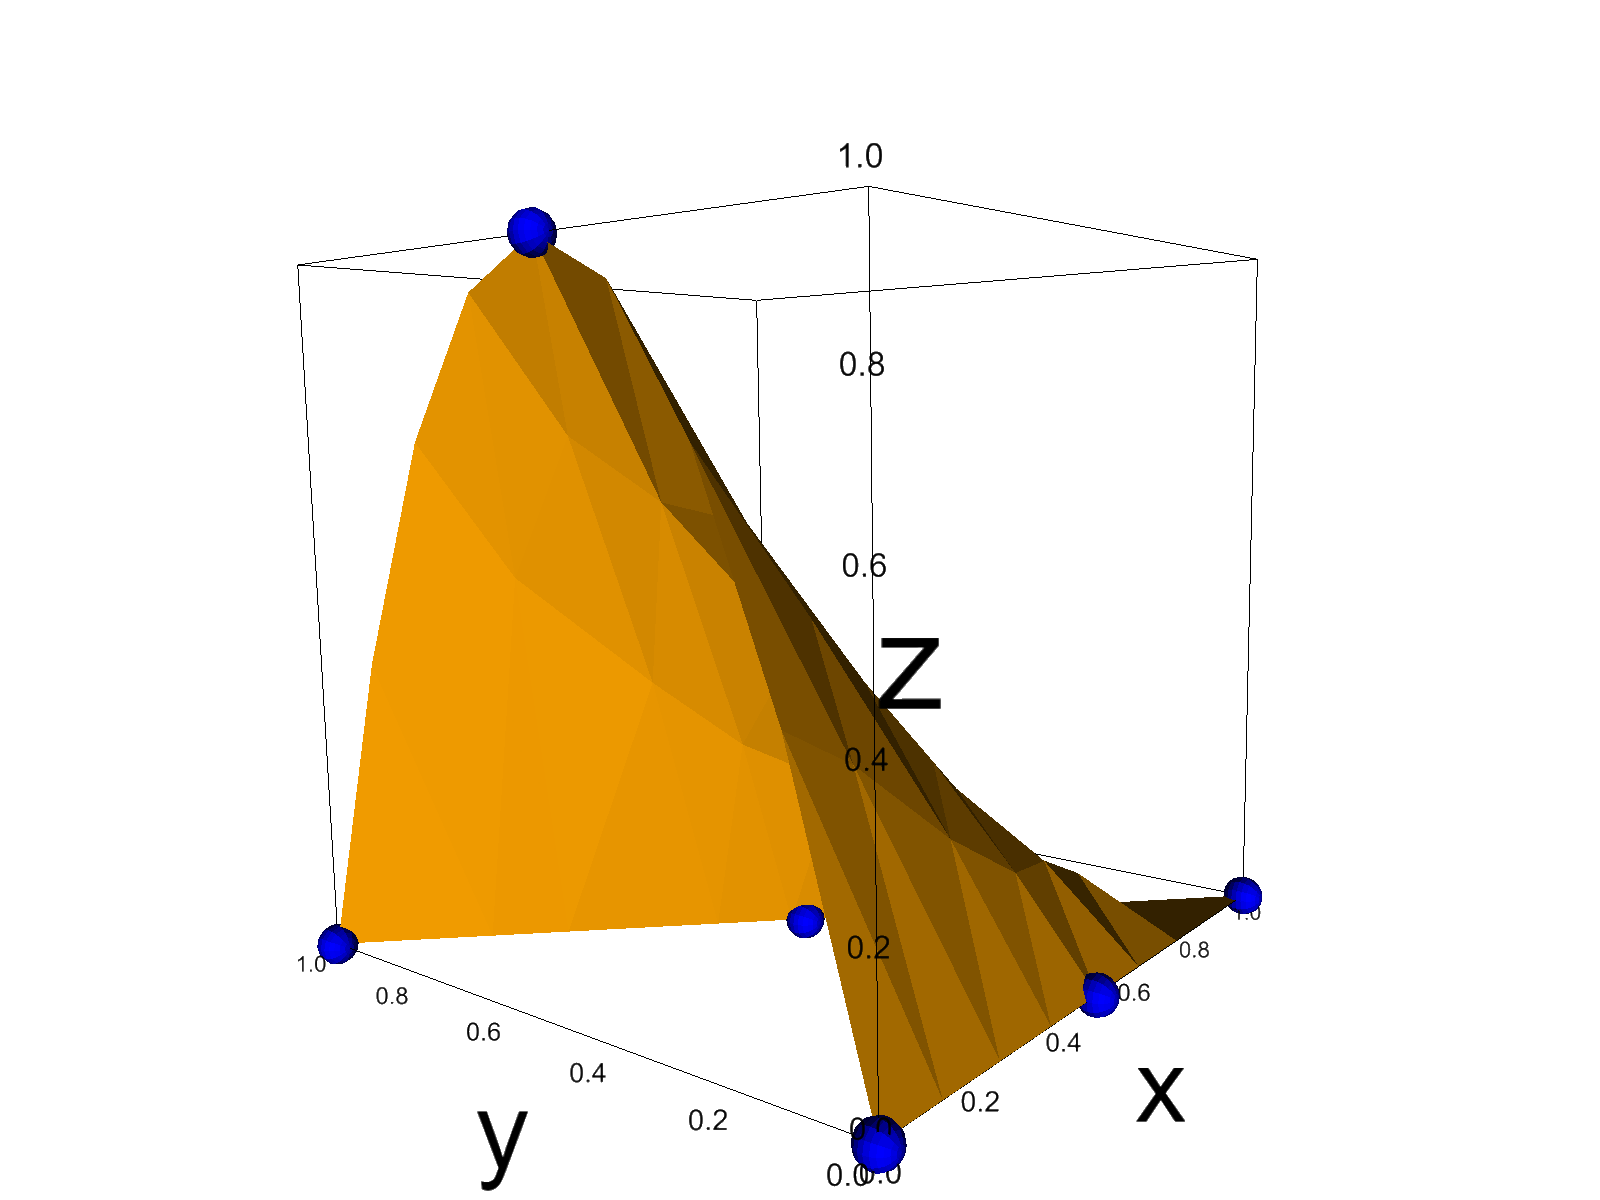
\includegraphics[width=\textwidth]{Pics/BasisFunc/triBasis4.png}
     \caption{\phi_4(x,y) = 4y(1-x-y),}
 \end{subfigure}
 \hfill
 \begin{subfigure}{0.5\textwidth}
     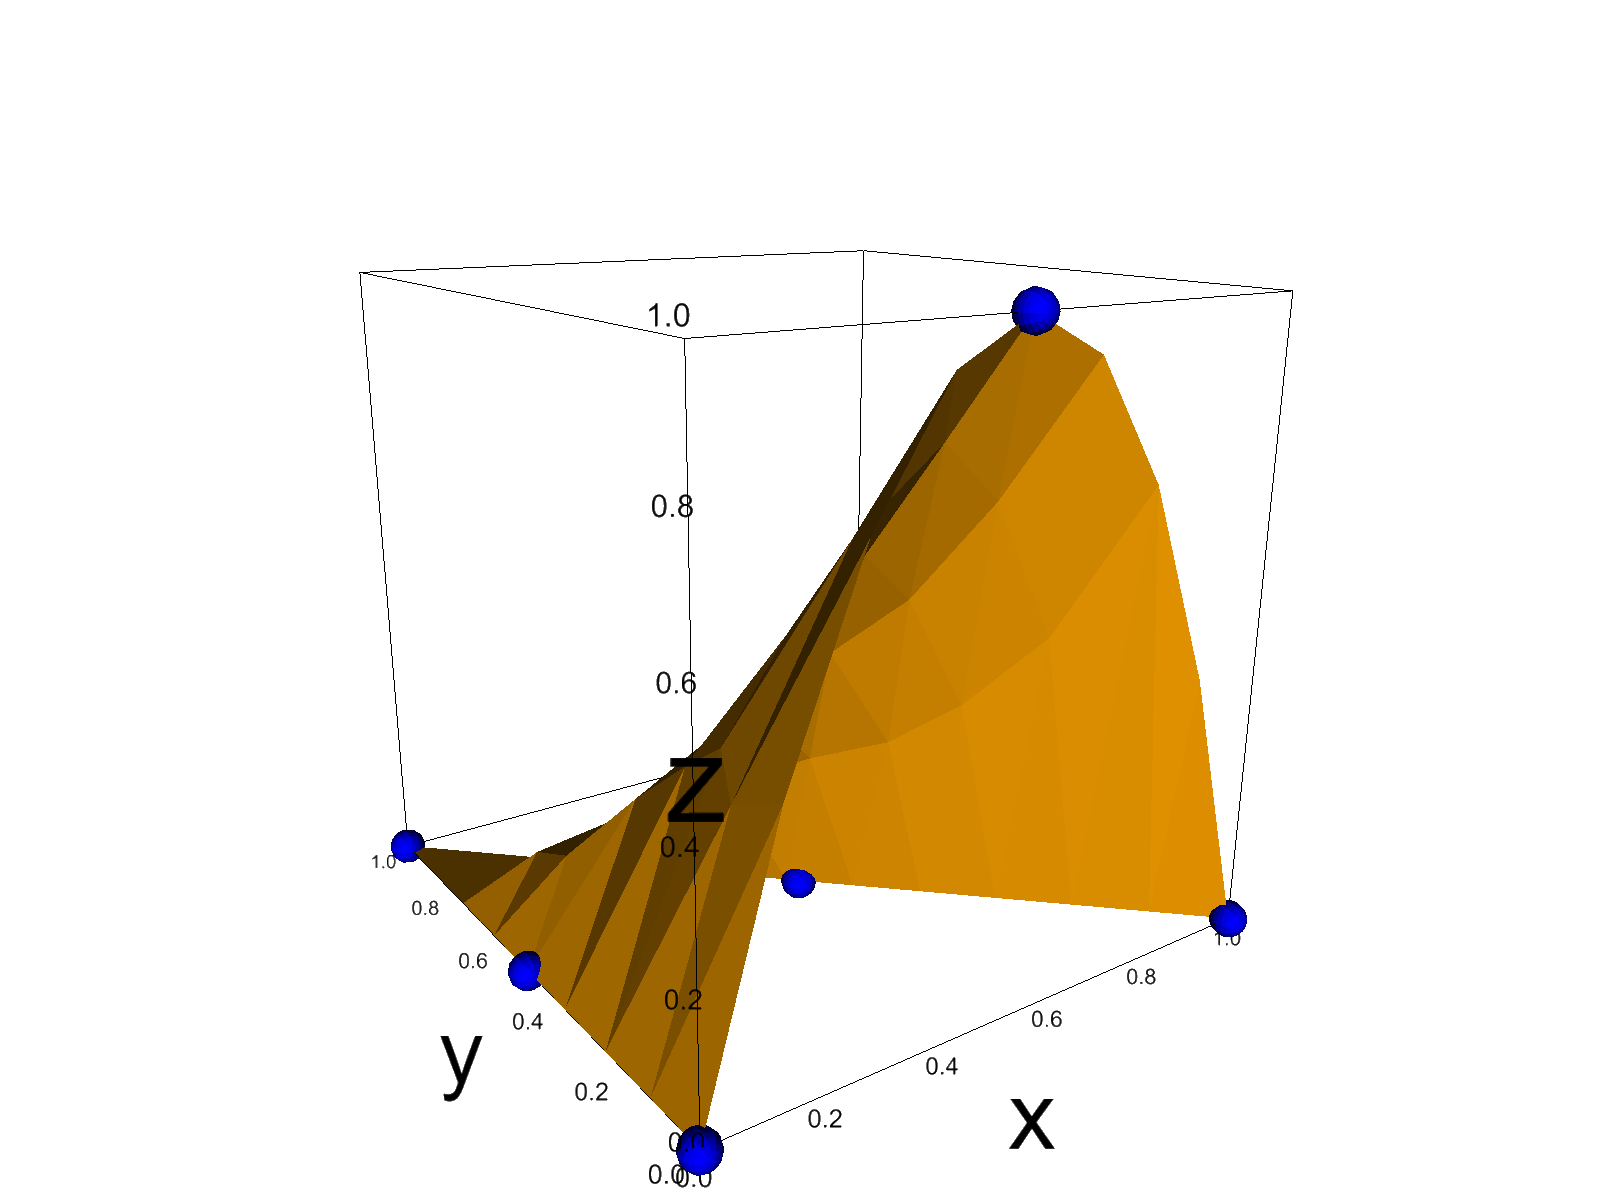
\includegraphics[width=\textwidth]{Pics/BasisFunc/triBasis5.png}
     \caption{\phi_5(x,y) = 4x(1-x-y),}
 \end{subfigure}
 \hfill
 \caption{Visual aids for the derivation of the Toroidal parameterisation.} \label{triBasisFuncs}
\end{figure}

\subsection{}
So why talking about it.

\subsection{Solve Linear System in Parrelle}

\end{document}